\section{実験結果}

測定した丸棒試験片について,$\Psi$と$2\theta$から,塑性変形前と後のA点,B点のそれぞれについて$\mathrm{sin}^2\Psi$ー$2\theta$線図を作成した.塑性変形前のA点,B点についての$\mathrm{sin}^2\Psi$ー$2\theta$線図を図\ref{fig:fig_BeforeRed},図\ref{fig:fig_BeforeBlack}にそれぞれ示す.また,塑性変形前のA点,B点についての$\mathrm{sin}^2\Psi$ー$2\theta$線図を図\ref{fig:fig_AfterRed},図\ref{fig:fig_AfterBlack}にそれぞれ示す.
\begin{figure}[htbp]
    \centering %中央揃え
    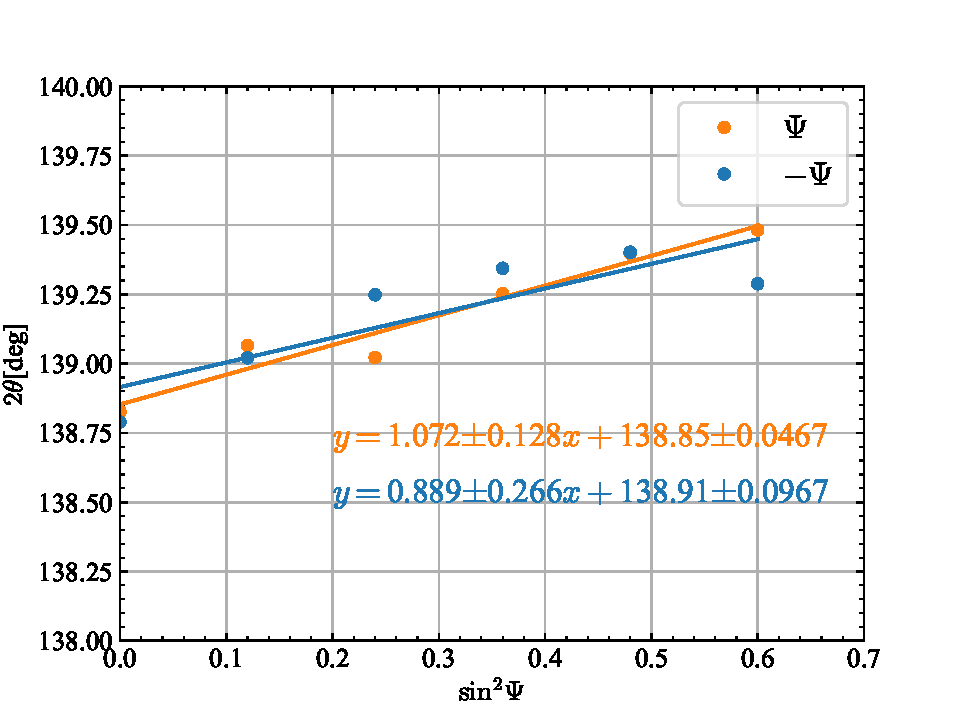
\includegraphics[width=100truemm,clip]{fig/fig_BeforeRed.pdf}
    \caption{$\mathrm{sin}^2\Psi$ー$2\theta$diagram at point A before plastic deformation.}
    \label{fig:fig_BeforeRed}
\end{figure}
\begin{figure}[htbp]
    \centering %中央揃え
    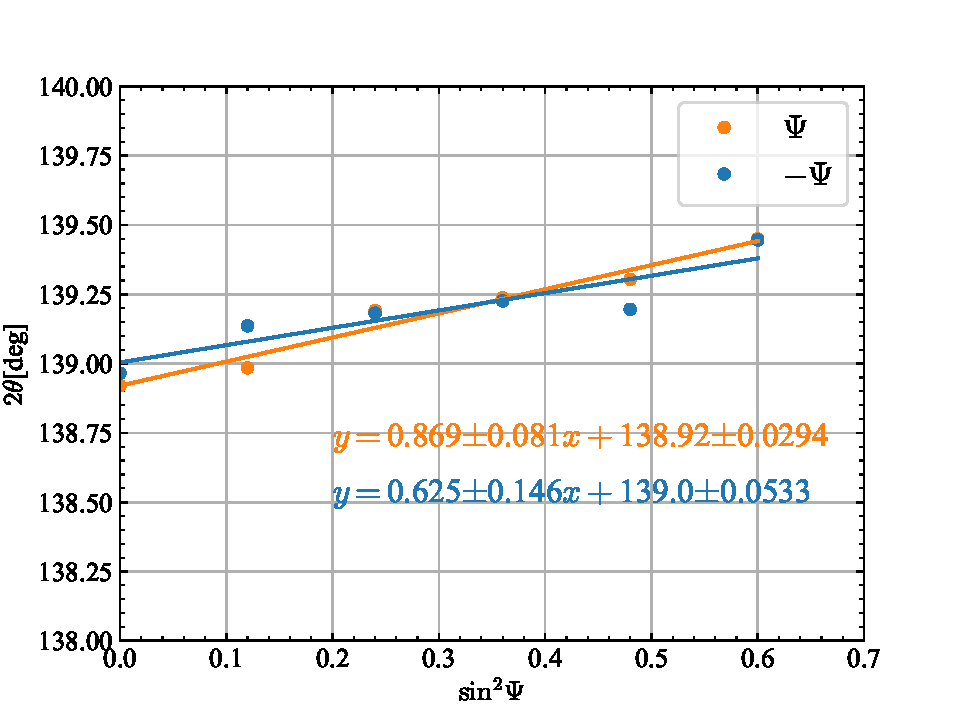
\includegraphics[width=100truemm,clip]{fig/fig_BeforeBlack.pdf}
    \caption{$\mathrm{sin}^2\Psi$ー$2\theta$diagram at point B before plastic deformation.}
    \label{fig:fig_BeforeBlack}
\end{figure}

\begin{figure}[htbp]
    \centering %中央揃え
    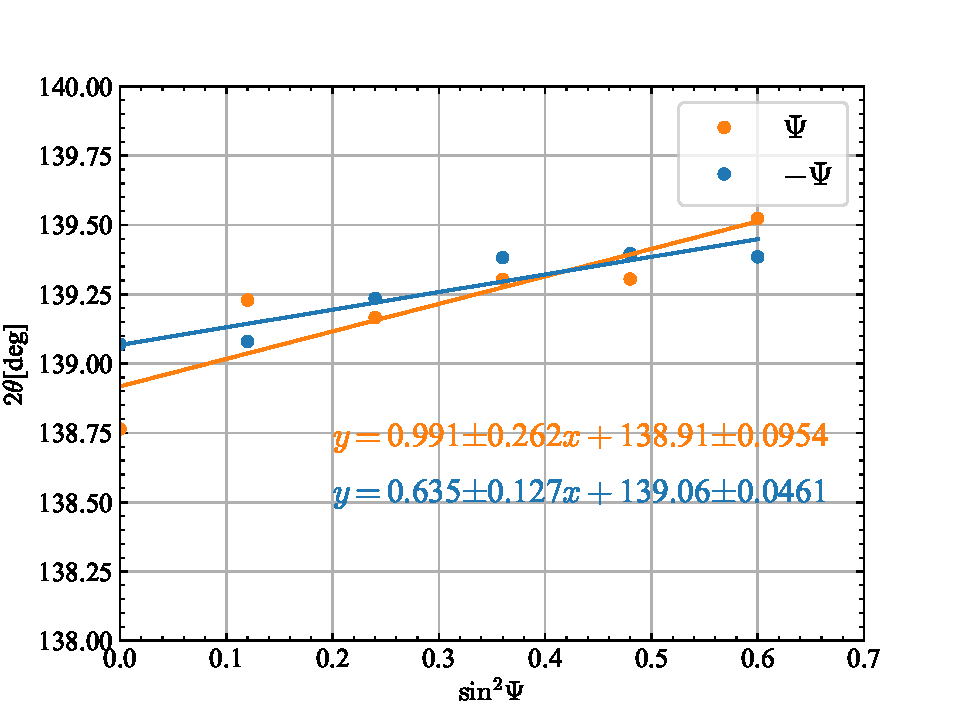
\includegraphics[width=100truemm,clip]{fig/fig_AfterRed.pdf}
    \caption{$\mathrm{sin}^2\Psi$ー$2\theta$diagram at point A after plastic deformation.}
    \label{fig:fig_AfterRed}
\end{figure}

\begin{figure}[htbp]
    \centering %中央揃え
    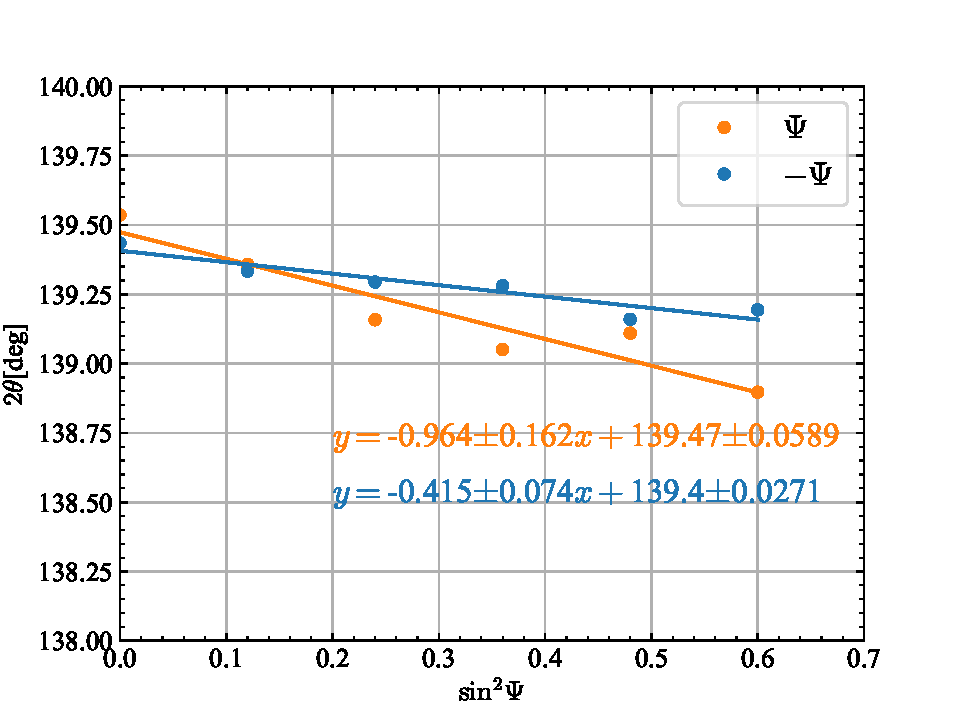
\includegraphics[width=100truemm,clip]{fig/fig_AfterBlack.pdf}
    \caption{$\mathrm{sin}^2\Psi$ー$2\theta$diagram at point B after plastic deformation.}
    \label{fig:fig_AfterBlack}
\end{figure}

\clearpage

図\ref{fig:fig_BeforeRed}から図\ref{fig:fig_AfterBlack}で得られた$\mathrm{sin}^2\Psi$ー$2\theta$線図から,式(\ref{eq:応力_x}),表\ref{tbl:応力定数表}を用いて,A点,B点それぞれの応力と信頼限界を求めた.表\ref{tbl:応力値と信頼限界}にA点,B点の応力値とその信頼限界を示す.


\begin{table}[htbp]
    \centering
    \caption{Stress values and their confidence limits at points A and B before and after plastic deformation, respectively.}
    \label{tbl:応力値と信頼限界}
    \scalebox{0.7}{
    \begin{tabular}{cccc}
    \hline
                                & 応力の最良推定値{[}MPa{]} & 上限信頼限界{[}MPa{]} & 下限信頼限界{[}MPa{]} \\ \hline
    Before bending point A (ψ)  & -312           & -349            & -274            \\ \hline
    Before bending point A (-ψ) & -258           & -336            & -181            \\ \hline
    Before bending point B (ψ)  & -253           & -276            & -229            \\ \hline
    Before bending point B (-ψ) & -182           & -224            & -139            \\ \hline
    After bending point A (ψ)   & -288           & -364            & -212            \\ \hline
    After bending point A (-ψ)  & -185           & -221            & -148            \\ \hline
    After bending point B (ψ)   & 280            & 233             & 327             \\ \hline
    After bending point B (-ψ)  & 121            & 99.0            & 142             \\ \hline
    \end{tabular}
    }
\end{table}